\renewcommand{\inputfile}{\version\ - edited 2008-06-26 stabOrder}
% $Author$ $Date$

%\section{Stability ordering of cycle expansions}
%\label{s-StabOrd}
% extracted from \Chapter{recycle}{30aug2006}{Cycle expansions}

\noindent
\index{cycle!expansion!stability ordered}
\index{stability!ordering!cycle expansions}
Most dynamical systems of interest have no finite grammar, so
at any order in $z$ a cycle
expansion may contain unmatched terms which do
not fit neatly into the almost canceling curvature corrections.
Similarly, for intermittent systems discussed
in \wwwcb,
curvature corrections are in general not small, so again the
cycle expansions may converge slowly.  For such systems
schemes which
% do not respect the topology of the flow, but
collect the
pseudo\-cycle terms according to some criterion other
than the topology of the flow may converge
more quickly than expansions based on the topological length.

All chaotic systems exhibit some degree of shadowing, and a
good truncation criterion should do its best to respect the shadowing
at least approximately.
If a long cycle is
shadowed by two or more shorter cycles and the flow is smooth, the period
and the action will be additive in sense that the period of the longer cycle is
approximately the sum of the shorter cycle periods.  Similarly,
stability is multiplicative, so shadowing is approximately preserved
by including all terms with pseudocycle stability
\beq
\left|\ExpaEig_{p_1}\cdots\ExpaEig_{p_k}\right| \leq \stabCutoff
\ee{StabCutoff}
and ignoring all more unstable pseudocycles.

Two such schemes for ordering cycle expansions which
approximately respect shadowing are truncations
by the pseudo\-cycle period (or action)
%\Preliminary{
%discussed in \refrem{r-BKconj},
%            }% end \Preliminary
and the stability ordering
that we shall discuss here.  In these schemes a \dzeta\ or a
\fd\ is expanded keeping all terms for which the period, action or stability
for a combination of cycles (pseudocycle) is less than a given cutoff.


Stability ordering was introduced by
Dahlqvist and Russberg\rf{DR91} in a study of chaotic dynamics for the
$(x^2y^2)^{1/a}$ potential.
%in the quantum case.
The presentation here is extracted from \wwwcb, and
follows the exposition of
Dettmann and Morriss\rf{DM97} for the Lorentz gas
which is hyperbolic but the symbolic dynamics is highly pruned, and
Dettmann and Cvitanovi\'c\rf{carl97int} for a family of intermittent maps.
In
%all of
the
%above
applications discussed in the above papers, the stability ordering
yields a considerable improvement over the topological length
ordering. In quantum chaos applications cycle expansion cancelations
are affected by the phases of pseudocycles (their actions), hence
{\em period ordering} rather than stability is frequently employed.

The two settings in which the stability ordering may be preferable to
\PC{add Berry-Keating somewhere}
the ordering by topological cycle length are the cases of bad grammar
and of intermittency.


\subsection{Stability ordering for good grammars}

We now  explore three
approaches to construction of a partition of
the \statesp\ of a unimodal map,
in the presence of weak, Gaussian noise, by
adopting the deterministic partitions by
\begin{itemize}
    \item preimages of the critical point
    \item kneading invariant of the critical point
    \item periodic orbit neighborhoods.
\end{itemize}

%\subsection{Skew Ulam map:}{ \label{exmp:SkewUlam}
%
    \PC{draw \reffig{f:skewUlam}!}
%
We shall refer to any unimodal map for which
the critical point $x_c$ is
mapped onto the unstable fixed point \cycle{0} as an ``Ulam'' map.
For Ulam maps of the critical point is preperiodic to fixed
point \cycle{0}, so the kneading invariant
is simply 1\cycle{0}, and it plays no further role in partitioning
of the \statesp.
As a model map on which to test different approaches
we take the ``skew Ulam" map\rf{AACII},
\beq
f(x)=\ExpaEig_0 x(1-x)(1-bx) \,\, , \quad
1/\ExpaEig_0  = x_c (1-x_c) (1-b x_c) \,.
\label{exmp:skew_Ulam}
\eeq
The $x_0=0$ fixed point \cycle{0} stability multiplier $\ExpaEig_0$
is fixed by condition $f(x_c)=1$, and $x_c$ as a  function
of $b$ fixed by $f'(x_c)=0$ condition.
The skew Ulam map
is a convenient starting point for testing
ideas about partitioning for several reasons:
\begin{itemize}
\item
The symbolic dynamics is a complete binary symbolic dynamics,
and the $n$th preimage
of the critical point generates a complete binary cover
of the unit interval.\PC{add refs}

\item
All cycles can be easily determined through a combination of
inverse iterations %, \refsect{s_inv_1d},
and the Newton method\rf{DasBuch}. %\refsect{s-Newton1d}.

\item
The quadratic contraction around the critical point
$x_c$ makes this  mapping {\em nonhyperbolic}.

\end{itemize}


In our numerical work we fix  $b=0.6$ (arbitrarily,
it is the value used in \refref{AACII}), so
$x_c =0.40456\dots$, and $\ExpaEig_0 = 5.4819\dots$ in
\refeq{exmp:skew_Ulam}.
% x_c=((1+b)-sqrt(1-b+b*b))/3 -> x_c =.40456678405103627197
% 1/\ExpaEig_0 = .18241823856341201233

%%%%%%%%%%%%%%%%%%%%%%%%%%%%%%%%%%%%%%%%%%%%%%%%%%%%%%%%%%%%%%%%
\begin{figure}
    % \vspace*{-5pt}
\begin{center}
	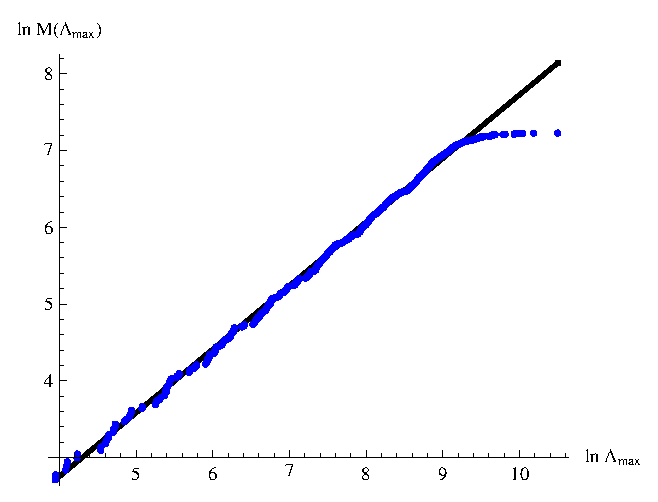
\includegraphics[width=0.75\textwidth]{figs/skewUlamEntropy}
\end{center}
\caption[Stability cutoff for skew Ulam map.]{
    {\small
The entropy $h = \ln M(\stabCutoff)/\ln\stabCutoff$ for the
the skew Ulam map \refeq{exmp:skew_Ulam}, stability partitioned \statesp,
is the slope of $\ln M(\stabCutoff)$ {\em vs.}  $\ln \stabCutoff$.
Here the set of all periodic orbits up to topological length $13$ for $b=0.6$
was generated and then ordered according to stability. From the linear
fit $h\simeq 0.830$.
        }}
\label{fig:logStabOrder1}
    % \vspace*{-5pt}
\end{figure}
%%%%%%%%%%%%%%%%%%%%%%%%%%%%%%%%%%%%%%%%%%%%%%%%%%%%%%%%%%%%%%%%%

Let $M(\stabCutoff)$
    \ES{Changed $M(\ln \stabCutoff)$ and $h(\ln \stabCutoff)$
        to $M(\stabCutoff)$ and $h(\stabCutoff)$ respectively.}
be the number of prime cycles whose stability is less than $\stabCutoff$.
For a chaotic system, $M$ is expected to grow exponentially with $ \stabCutoff)$ and
the rate of the growth is the
``entropy" $h (\stabCutoff) = \ln M(\stabCutoff)/\ln\stabCutoff$
is expected to go to a value $h$ as $\stabCutoff \to \infty$.
This value is probably the Kolmogorov entropy.
    \PC{Vaggelis, read up
        on Kolmogorov entropy, and examples of it for 1$\dmn$ mappings}
For the
the skew Ulam map \refeq{exmp:skew_Ulam}, stability
partitioned \statesp,
$h$ is the slope of
the $\ln M(\stabCutoff)$ {\em vs.}
$\ln \stabCutoff)$
the Kolmogorov entropy (maybe - see Eq. (88) in \refref{AACI}, which
is probably not the correct definition, either) evaluated from
the zeta functions \refeq{??} is plotted in \reffig{fig:logStabOrder1}.

%%%%%%%%%%%%%%%%%%%%%%%%%%%%%%%%%%%%%%%%%%%%%%%%%%%%%%%%%%%%%%%
\begin{figure}
    \vspace*{-5pt}
\begin{center}
	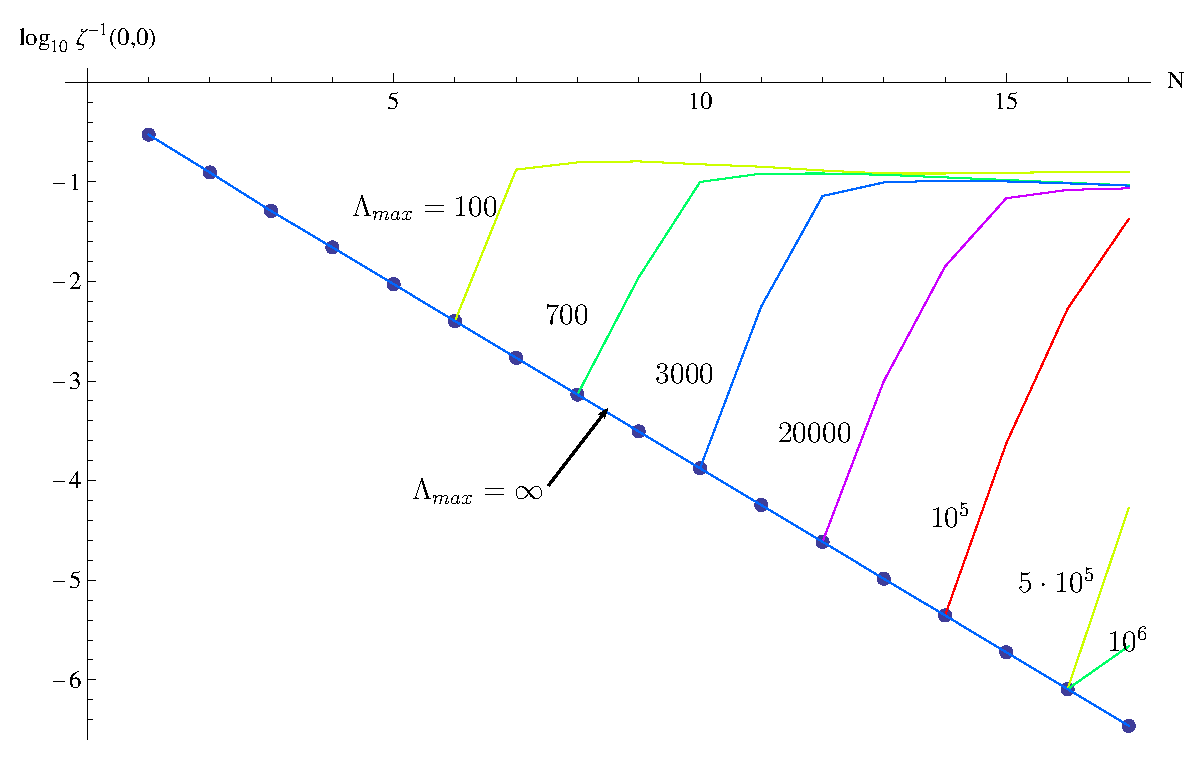
\includegraphics[width=0.75\textwidth]{figs/skewUlamZeta}
\end{center}
\caption[flow conservation relation for skew Ulam map]
    {
Consistency check of flow conservation relation \refeq{prob-cons}
for skew Ulam map  \refeq{exmp:skew_Ulam} for $b=0.6$.
Here all cycles up to topological length $13$ were found through
inverse iteration and the dynamical zeta function $1/\zeta(0,0)$ was evaluated
from \refeq{prob-cons-zeta} with stability cutoff $\stabCutoff$ as
in \refeq{StabCutoff}.
	}
\label{fig:zetaStabOrder1}
    \vspace*{-5pt}
\end{figure}
%%%%%%%%%%%%%%%%%%%%%%%%%%%%%%%%%%%%%%%%%%%%%%%%%%%%%%%%%%%%%%%%
\PC{ For a plot  of all
pseudocycles contributing to
$\ln|1/\zeta(0,0)|$, fluctuations to large negative values are OK;
$1/\zeta(0,0)$ is presumably constantly changing sign, so every so often you
get it close to 0. You'll probably also interpret the two parallel lines
on the top as partially not shadowed cycles with lots of zeros.
\\ ===
In \refref{AACII} it is explained why
you should replace the $\ExpaEig_{0}$ in the $1/\zeta(0,0)$ by
by $\ExpaEig_{0}^{1/2}$. Check whether stabilities of
your cycles with itineraries
with long sequences of 0's agree with my calculation.
\\ === Starting with $\ln M(\stabCutoff) \approx 7$ the
appearance of higher errors is suspicious. To me it looks like
your cycle stabilities might be getting inaccurate, perhaps because inverse
iteration is not as accurate as multi-shooting Newton.
\\ === by
$\ln M(\stabCutoff) \approx 9$ there appears to be
something numerically wrong with the calculation, because $\ln|1/\zeta(0,0)|$
cannot start increasing.
\\ === Are you sure that your $\stabCutoff$ is smaller than the
{\em least unstable} 13-cycle $\ExpaEig_p$? Missing those would explain
your troubles starting with $\stabCutoff \approx 9.2$
\\ \bf{ES:} This is what happens. Can we use this plot to illustrate that
	once you miss some cycles $\ln|1/\zeta(0,0)|$ starts increasing?
\\ === read \refsect{s-Smoothing}; do you agree with the imperfect shadowing
error estimates? Check them numerically.
}

\subsection{Stability ordering for bad grammars}

For generic flows it is often not clear what
% Poincar\'{e} section should be used, and how it should be
partition of the {\statesp} generates the ``optimal''
symbolic dynamics.  Stability ordering
does not require understanding dynamics in such detail:
if you can find the cycles, you can use
stability ordered cycle expansions.
Stability truncation
% requires only that all cycles up to given
% stability cutoff be determined, without
% requiring detailed understanding of the topology of the
% flow and symbolic dynamics. It
is thus
%much
easier to implement for
a generic dynamical system than the
curvature expansions
\PC{refer here to the thesis section} %\refeq{curvbin}
which rely on finite subshift approximations
to a given flow.

Cycles can be detected numerically by
searching a long trajectory for near recurrences.
The long trajectory method for detecting cycles
\PC{refer here to the thesis section} %\refsect{s_long_time}
preferentially finds
the least unstable cycles, regardless of their topological length.
Another practical advantage of the method (in contrast to
Newton method searches)
is that it only finds
cycles in a given connected ergodic component of {\statesp},
ignoring  isolated cycles or other ergodic regions
elsewhere in the {\statesp}.

Why should stability ordered cycle expansion of a \dzeta\ converge
better than the rude trace formula
\PC{explain better}
\refeq{LevelAver}?
\PC{refer here to the thesis equation}
The argument has essentially already been laid out in
\refsect{s-Shadow}:
\PC{refer here to the thesis equation}
in truncations that respect shadowing most of
the pseudocycles appear in shadowing combinations and nearly cancel,
while only the relatively small subset affected by the longer and
longer pruning rules is not shadowed. So the error is typically
of the order of $1/\ExpaEig$, smaller by factor $e^{hT}$ than the
\PC{refer here to the thesis equation}
trace formula
%\refeq{levl-sumHOA}
\refeq{LevelAver}
error, where $h$ is the entropy and
$T$ typical cycle length for cycles of stability  $\ExpaEig$.
\PC{Incorporate Grassberger's dimension of the Cantor set of pruning rules}

\subsection{Smoothing}
\label{s-Smoothing}

The breaking of exact shadowing cancellations deserves further comment.
Partial shadowing which may be present can be (partially) restored by smoothing
the stability ordered cycle expansions by replacing the
$1/\ExpaEig$ weight for each term with
pseudocycle stability
$\ExpaEig=
\ExpaEig_{p_1}\cdots\ExpaEig_{p_k}$ by $f(\ExpaEig)/\ExpaEig$.
Here, $f(\ExpaEig)$ is a monotonically decreasing function from $f(0)=1$ to
$f(\stabCutoff)=0$.  No smoothing corresponds to a step function.
\PC{I do not believe yet that this is significant improvement}

A typical ``shadowing error'' induced by the cutoff is due to two
pseudocycles of stability $\ExpaEig$ separated by $\Delta\ExpaEig$, and
whose contribution is of opposite signs.
Ignoring possible weighting factors the magnitude of the resulting term
is of order
$1/\ExpaEig-1/(\ExpaEig+\Delta\ExpaEig)
\approx\Delta\ExpaEig/\ExpaEig^2$.
% \PC{I think this is wrong - error is of order $1/\ExpaEig$?
% this estimate is true for the intermittent case only?}
With smoothing there is an
extra term of the form $f'(\ExpaEig)\Delta\ExpaEig/\ExpaEig$, which we
want to minimize.  A reasonable guess might be to keep $f'(\ExpaEig)/\ExpaEig$
constant and as small as possible, that is
\[
f(\ExpaEig)=1-\left(\frac{\ExpaEig}{\stabCutoff}\right)^2
\]

The results of a stability ordered expansion
\refeq{StabCutoff}
should always be tested for
robustness by varying the cutoff  $\stabCutoff$.
If this introduces significant variations,
smoothing is probably necessary.
% It is also necessary in any scheme which
% attempts to extrapolate results to infinite $\stabCutoff$.

%%%%%%%%%%%%%%%%%%%%%%%%%%%%%%%%%%%%%%%%%%%%%%%%%%%%%%%%%%%%%%%%
\begin{figure} \label{fig:logStabOrder1}
\begin{center}
plot here % \includegraphics[width=0.75\textwidth]{../figs/nameMe}
\end{center}
\caption[The leading eigenvalue convergence for the logistic map]
        {
The leading eigenvalue $\ln | s_0^{(N)} - s_0|$
convergence for the
logistic map (??), plotted {\em vs.} $ln N$.
The convergence of
(a)  the first $\eigenvL_0 = - \gamma = ???$
and
(b)  the second $\eigenvL_1 = ???$ eigenvalues
of the
\FP. Plotted:
$\ln |\eigenvL_\alpha^{(N)}-\eigenvL_\alpha^{\infty|}$
as a function of $\ln N$,
the number of partition intervals $N$.
In the binary
logistic map partition, with the $2^n$ intervals,
$\ln N= n \ln 2$ for the skew Ulam map \refeq{exmp:skew_Ulam}.
$\eigenvL_\alpha$ is estimated as a limit
$\eigenvL_\alpha^{(\infty)}$ from the computed
$\ln |\eigenvL_\alpha^{(N)}|$.
        }
    % \vspace*{-5pt}
\end{figure}
%%%%%%%%%%%%%%%%%%%%%%%%%%%%%%%%%%%%%%%%%%%%%%%%%%%%%%%%%%%%%%%%%%


The leading eigenvalue convergence
$\ln |\eigenvL_0^{(N)} - \eigenvL_0|$ is plotted in
\reffig{fig:logStabOrder1} as a function of
$ln N$,
the number of intervals $N$ is $N = 2^{n}$
for the for the skew Ulam map \refeq{exmp:skew_Ulam},
$N =e^{n h_n}$ for a pruned logistic map, and $N = N(\stabCutoff)$
for the stability ordered cycle expansion.

Plotted:
$\ln |\eigenvL_\alpha^{(N)}-\eigenvL_\infty|$
as a function of $\ln N$,
the number of partition intervals $N$.
In the deterministic
Ulam map partition, with the $2^n$ intervals,
$\ln N= n \ln 2$.
$\eigenvL_\alpha$ is estimated as a limit
$\eigenvL_\alpha^{(\infty)}$ from the computed
$\ln |\eigenvL_\alpha^{(N)}|$.



\subsection{Topological entropy, Lyapunov exponents}
\label{s-StOrdKS}

Compute here the topological entropy for the logistic map, first
as in \wwwcb, ``Counting" chapter, and then as a function of
$\ln \stabCutoff = - \ln \epsilon$, where $ \epsilon$ is the
effective unit interval discretization.
Compare the two in
\reffig{fig:EntrStabOrder1}.

I believe
$h_K = \lim_{{\stabCutoff} \to \infty} N(\stabCutoff)/\ln \stabCutoff$
is probably the Kolmogorov, or metric entropy, the lower bound on
$h$ computed as infimum of all possible \statesp\ partitionings.


%%%%%%%%%%%%%%%%%%%%%%%%%%%%%%%%%%%%%%%%%%%%%%%%%%%%%%%%%%%%%%%%
\begin{figure}\label{fig:EntrStabOrder1}
\begin{center}
plot here % \includegraphics[width=0.75\textwidth]{../figs/nameMe}
\end{center}
\caption[Entropy convergence for the logistic map]{
The entropy $\ln | h^{(N)} - h|$
convergence for the
logistic map (??), plotted {\em vs.} $ln N$
for the binary and the stability (Kolmogorov) \statesp\ partitioned
topological zeta functions.
        }
\end{figure}
%%%%%%%%%%%%%%%%%%%%%%%%%%%%%%%%%%%%%%%%%%%%%%%%%%%%%%%%%%%%%%%%%%



\subsection{Stability ordering for KS cycles}
\label{s-StOrdKS}

In this section we attempt to numerically check the
flow conservation sum rule \refeq{prob-cons} for \KS\ equation with $L=22$ 
using a set of $~10000$ periodic and $~10000$ relative
periodic orbits  computed by Ruslan L. Davidchack\rf{Davidchack_priv}.
In reduced space both \rpo s and pre-\po s are periodic so they should
entered in the same way in dynamical zeta function calculations\ES{Or do we have to
count some multiplicity due to $\Dn{1}$ differently? There is a copy of any rpo
due to $\Dn{1}$ but we also only consider $1/2$ of each periodic orbit, so I think
we are fine.}. the dynamical zeta function $1/\zeta(0,0)$ was evaluated
from \refeq{prob-cons-zeta} with stability cutoff $\stabCutoff$ as
in \refeq{StabCutoff}. After $\stabCutoff\simeq1200$
dynamical zeta function grows, indicating that we are missing some cycles.
To find them we will really have to understand the geometry of the flow.

%%%%%%%%%%%%%%%%%%%%%%%%%%%%%%%%%%%%%%%%%%%%%%%%%%%%%%%%%%%%%%%
\begin{figure}
    \vspace*{-5pt}
\begin{center}
	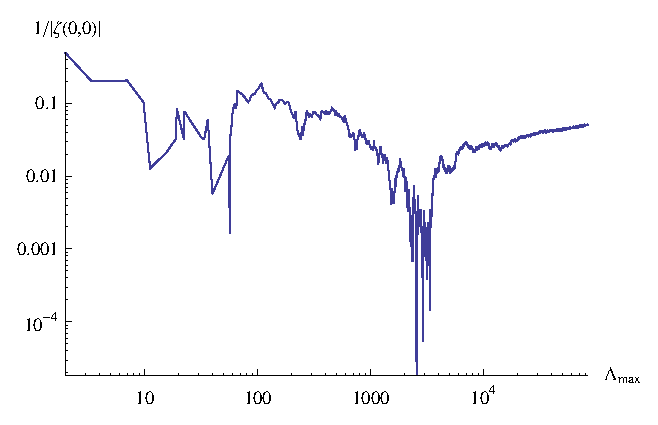
\includegraphics[width=0.75\textwidth]{../figs/ksStabOrder5000}
\end{center}
\caption[flow conservation relation for KSe, $L=22$]
    {
Consistency check of flow conservation relation \refeq{prob-cons}
for \KS\ equation \refeq{ks} for $L=22$.
Here the dynamical zeta function $1/\zeta(0,0)$ was evaluated
from \refeq{prob-cons-zeta} with stability cutoff $\stabCutoff$ as
in \refeq{StabCutoff}. The maximum stability cutoff shown corresponds
to using the $5000$ least unstable cycles in the set.
	}
\label{fig:zetaStabOrderKS22}
    \vspace*{-5pt}
\end{figure}
%%%%%%%%%%%%%%%%%%%%%%%%%%%%%%%%%%%%%%%%%%%%%%%%%%%%%%%%%%%%%%%%



\subsection{Stability ordering for intermittent flows}
\label{s-StOrdInterm}

\index{stability!ordering!intermittent flows}
\index{intermittency!stability ordering}
\PC{use what you need from this section, remove the rest}
Longer but less unstable cycles can give larger contributions
to a cycle expansion than short but highly unstable cycles.
In such situation truncation by length may require
an exponentially large number of very unstable cycles before a significant
longer cycle is first included in the expansion.
This situation is best illustrated by intermittent maps
\PC{add figure}
that we shall study in detail in \wwwcb, the simplest
of which is the Farey map
\PC{replace by your logistic map}
\beq
f(x)=\left\{\begin{array}{ccc}
f_0=x/(1-x) & \quad 0\leq x\leq 1/2& \\
f_1=(1-x)/x & \quad 1/2\leq x\leq 1& \,.
\end{array}
\right.
\ee{e:fareymap}

For this map the symbolic dynamics
is of complete binary type, so lack of shadowing is not due to
lack of a finite grammar, but rather to the
intermittency caused by the existence of the marginal fixed point $x_0=0$,
for which the stability equals
$\ExpaEig_0=1$.  This fixed point does not
participate directly in the dynamics and is omitted from cycle
expansions.  Its presence is felt in
the stabilities of neighboring cycles with $n$ consecutive repeats
of the symbol $0$'s whose stability falls of only as
% a power law
$\ExpaEig\sim n^2$, in contrast to
the most unstable cycles with $n$ consecutive $1$'s which  are
exponentially unstable, $|\ExpaEig_{01^n}|\sim[(\sqrt{5}+1)/2]^{2n}$.

The symbolic dynamics
is of complete binary type. A quick count in the style
of \wwwcb %\refsect{s-CountPrimes}
leads to a total of
74,248,450 prime cycles of length 30 or less, not including the marginal
point $x_0=0$. Evaluating a cycle expansion to this order
would be no mean computational feat.  However, the least unstable cycle
omitted has stability of roughly
$\ExpaEig_{10^{30}} \sim 30^2=900$, and so amounts to
a $0.1\%$ correction.  The situation may be much worse than this estimate
suggests, because the next, $10^{31}$
cycle contributes a similar amount, and could
easily reinforce the error.  Adding up all such omitted terms, we arrive
at an estimated error of about $3\%$,  for a cycle-length truncated
cycle expansion
based on more than $10^9$ pseudocycle terms! On the other hand,
truncating by stability at say $\stabCutoff=3000$,
only 409 prime cycles suffice to attain the same
accuracy of about $3\%$ error, \reffig{fig:logStabOrder}.

As the Farey map maps the unit interval onto itself, the leading eigenvalue of
the \FPoper\ should equal $\eigenvL_0=0$, so
$1/\zeta(0)=0$. Deviation from this exact result serves as an indication
of the convergence of a given cycle expansion.
The errors of different truncation
schemes are indicated in \reffig{fig:logStabOrder}.
We see that topological length truncation schemes are hopelessly
\PC{ why is error in \reffig{fig:logStabOrder}larger when smoothed?}
bad in this case; stability length truncations are somewhat better,
but still rather bad.

%%%%%%%%%%%%%%%%%%%%%%%%%%%%%%%%%%%%%%%%%%%%%%%%%%%%%%%%%%%%%%%%
\begin{figure} 
\begin{center}
	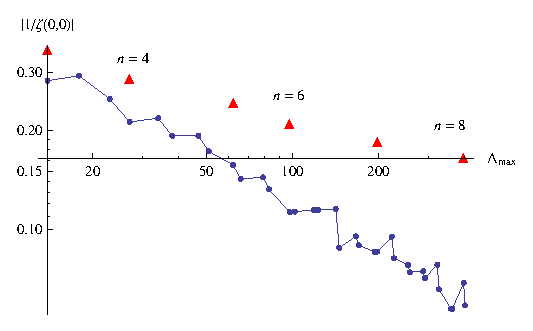
\includegraphics[width=0.75\textwidth]{figs/fareyZeta}
\end{center}
\caption[Cycle expansion truncation schemes for the Farey map]
        {
Comparison of cycle expansion truncation schemes for the
Farey map \refeq{e:fareymap}.
the deviation of the truncated cycles
expansion for $|1/\zeta_\nCutoff(0)|$ from the exact
flow conservation value $1/\zeta(0)=0$ is a measure of the accuracy of the
truncation.  The jagged
line is logarithm of the stability ordering
truncation error; the triangles indicate the error
due the topological length truncation, with
the maximal cycle length $\nCutoff$ shown.
They are placed along the stability cutoff axis at points determined
by the condition that the total number of cycles is the same for both
truncation schemes.
        }
\label{fig:logStabOrder}
\end{figure}
%%%%%%%%%%%%%%%%%%%%%%%%%%%%%%%%%%%%%%%%%%%%%%%%%%%%%%%%%%%%%%%%%%
